\documentclass[8pt]{beamer}

\usetheme{Copenhagen}
\usecolortheme{beaver}
\usepackage[small,center]{caption}
\usepackage{times}
\usefonttheme{structurebold}
\usepackage[english]{babel}
\usepackage{pgf,pgfarrows,pgfnodes,pgfautomata,pgfheaps}
\usepackage{amsmath,amssymb}
\usepackage{amsxtra}

\usepackage{caption}

\newcommand{\leftd}[1]{{\color{red} \bar{#1}}}
\newcommand{\interface}[2]{{\color{blue}{#1}_I(#2)}}
\newcommand{\leftdd}[2]{{\color{red} \bar{#1}(\bar{#2})}}
\newcommand{\leftFourier}[1]{{\color{red} \hat{#1}}}
\newcommand{\leftFourierTwo}[2]{{\color{red} \hat{#1}(\hat{#2})}}
\newcommand{\divergence}{\mathrm{div}}

\newcommand*{\vcenterimage}[1]{\vcenter{\hbox{\includegraphics[width=2in]{#1}}}}
\newcommand*{\vcenterarrow}{\vcenter{\hbox{$\Longrightarrow$}}}


\definecolor{RPIred}{rgb}{ 0.87,0.12, 0.20}
\definecolor{ballblue}{rgb}{0.13, 0.67, 0.8}
\definecolor{lightgray}{rgb}{0.83, 0.83, 0.83}
\setbeamercolor{block title}{bg=lightgray,fg=RPIred}
\setbeamercolor{block body}{bg=white,fg=black}
\setbeamercovered{dynamic}
\setbeamercolor*{item}{fg=RPIred}

\captionsetup[subfigure]{labelformat=empty}
\captionsetup[figure]{labelformat=empty}
\setbeamertemplate{navigation symbols}{}
\setbeamertemplate{footline}[frame number]
\begin{document}

\frame{
\title{\Large Decreasing Energy Aliasing in POD-ROMs}

\author{{\Large David Wells \\\vspace{0.1in} Rensselaer Polytechnic Institute}\\
\vspace{0.2in} {In collaboration with:\\{}T. Iliescu (VT), V. John (WIAS), S. Giere (WIAS)}}

\date{June 28, 2017\\{} Conference on Classical and Geophysical Fluid Dynamics}

\begin{figure}[h]
\centering
\includegraphics[width=1.5in]{RPI_letterhead.pdf}
 \end{figure}%

\vspace{-0.2in}
\titlepage
}

% vector notation
\newcommand{\va}{\vec{a}}
\newcommand{\bb}{\vec{b}}
\newcommand{\cc}{\vec{c}}
\newcommand{\ff}{\vec{f}}
\newcommand{\nn}{\vec{n}}
\newcommand{\uu}{\vec{u}}
\newcommand{\ww}{\vec{w}}
\newcommand{\xx}{\vec{x}}
\newcommand{\twoVector}[2]{\begin{bmatrix} #1 \\ #2 \end{bmatrix}}
\newcommand{\threeVector}[3]{\begin{bmatrix} #1 \\ #2 \\ #3 \end{bmatrix}}
\newcommand{\twoVectorT}[2]{\begin{bmatrix} #1 & #2 \end{bmatrix}}
\newcommand{\threeVectorT}[3]{\begin{bmatrix} #1 & #2 & #3 \end{bmatrix}}
\newcommand{\fourVectorT}[4]{\begin{bmatrix} #1 & #2 & #3 & #4 \end{bmatrix}}
\newcommand{\vr}{\vec{v}_r}

% bold commands
\newcommand{\bx}{{\mathbf x}}
\newcommand{\by}{{\mathbf y}}

% integral notation
\newcommand{\dxx}{\,d\xx}
\newcommand{\dll}{\,d\vec{l}}
\newcommand{\intO}{\int_\Omega}

\newcommand{\sumT}{\sum_{T\in \mathcal{T}_h}}
\newcommand{\intT}{\int_T}
\newcommand{\Th}{\mathcal{T}_h}

% typesetting
\newcommand{\todo}[1]{{\color{red}#1}}
\newcommand{\eg}{e.g., }
\newcommand{\ie}{i.e., }
\newcommand{\frameBoxShort}[1]{\begin{center} \begin{minipage}{0.8\textwidth}\begin{center}\fbox{#1}\end{center}\end{minipage} \end{center}}
\newcommand{\frameBox}[1]{\noindent\begin{center} \begin{minipage}{\textwidth}\framebox{#1}\end{minipage} \end{center}}

% SUPG notation
\newcommand{\eps}{\varepsilon}
\newcommand{\SDNorm}[1]{||| #1 |||_{SD}}
\newcommand{\SDRNorm}[1]{||| #1 |||_{\mathrm{SUPG}, r}}
\newcommand{\SDInner}[2]{a(#1, #2)_{SD}}
\newcommand{\SUPGRInner}[1]{a(#1)_{\mathrm{SUPG}, r}}
\newcommand{\half}{1/2}
\newcommand{\threehalves}{3/2}

% functional analysis
\newcommand{\abs}[1]{\ensuremath{\left| #1 \right|}}
\newcommand{\Norm}[1]{\ensuremath{\| #1 \|}}
\newcommand{\Norms}[1]{\ensuremath{\left\| #1 \right\|}}
\newcommand{\Seminorm}[1]{\ensuremath{| #1 |}}
\newcommand{\Seminorms}[1]{\ensuremath{\left| #1 \right|}}
\newcommand{\Langles}[1]{\left\langle#1\right\rangle}
\newcommand{\Brackets}[1]{\ensuremath{\left\{#1\right\}}}

% POD notation
\newcommand{\snapsum}{\sum_{n = 0}^{R - 1}} % sum of snapshots
\newcommand{\remainder}[1]{\sum_{#1 = r}^{R - 1}} % sum from r to R - 1
\newcommand{\podsum}[1]{\sum_{#1 = 0}^{r - 1}} % sum of POD vectors
% (uh(., tl), phij(.))
\newcommand{\inl}[1]{\Langles{u_n, \phi_{#1}}}
\newcommand{\podvec}{\vec{\varphi}}
\newcommand{\OO}{\mathcal{O}}

% NS notation
\newcommand{\reinv}{\dfrac{1}{Re}}

% NS and POD notation
\newcommand{\usteady}{\uu_s}
\newcommand{\podgalerkin}{\usteady + \podsum{j} a_j(t) \podvec_j(\xx)}
\newcommand{\podgalerkinx}{\uu_{s0} + \podsum{j} a_j(t) \varphi_{j0}(\xx)}

\newcommand{\evaluateBetween}[2]{\, \biggr\rvert_{#1}^{#2}}
\newcommand{\RR}{\mathbb{R}}
\newcommand{\mult}{\dfrac{1}{(2 \pi)^{n/2}}}
\newcommand{\multt}{\dfrac{1}{\sqrt{2 \pi}}}

% filtering notation
\newcommand{\FF}{\mathcal{F}}


\begin{frame}
    \frametitle{Outline}
    \begin{itemize}
    \item[$\blacksquare$] Governing Equations                                 \\
    \item[$\blacksquare$] A Little on Streamline-Upwind Petrov-Galerkin (SUPG)\\
    \item[$\blacksquare$] The SUPG-ROM                                        \\
    \item[$\blacksquare$] Numerical Results                                   \\
    \item[$\blacksquare$] Summary                                             \\
    \end{itemize}
\end{frame}

\section{Governing Equations}
    \begin{frame}
        \frametitle{Convection-Diffusion-Reaction Equation}
        There are a few relevant model problems:
        \begin{align}
            u_t - \varepsilon \Delta u + \vec{b} \cdot \nabla u + c u &= f    \\
            -\varepsilon \Delta u + \vec{b} \cdot \nabla u + c u      &= f
        \end{align}
        \begin{itemize}
            \item \(\varepsilon \ll 1\) and \(\varepsilon \ll h\)
            \item Small diffusion implies wavelike behavior
                  (\emph{convection-dominated}): the relevant length scale is
                  \(O(\sqrt{\varepsilon})\), which may be too small to resolve.
        \end{itemize}
    \end{frame}

    \begin{frame}
        \frametitle{Convection-Diffusion-Reaction Equation}
        \begin{center}
            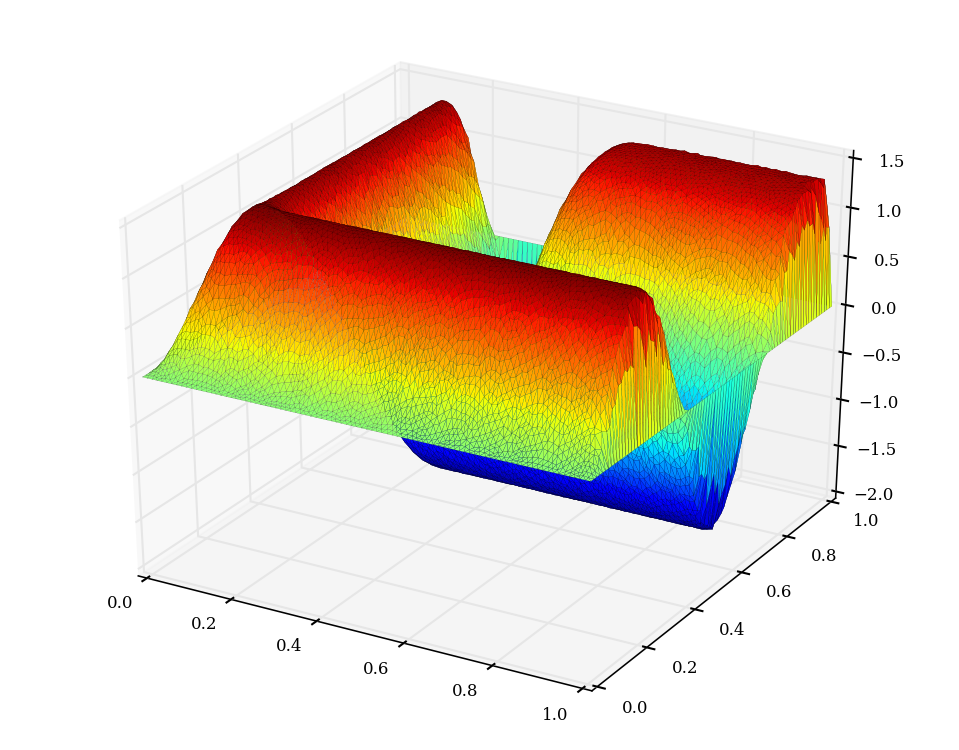
\includegraphics[width=3in]{Pictures/CDR/cdr_vector_3.png}

            Third POD vector.
        \end{center}
    \end{frame}

    \begin{frame}
        \frametitle{Convection-Diffusion-Reaction Equation}
        \begin{center}
            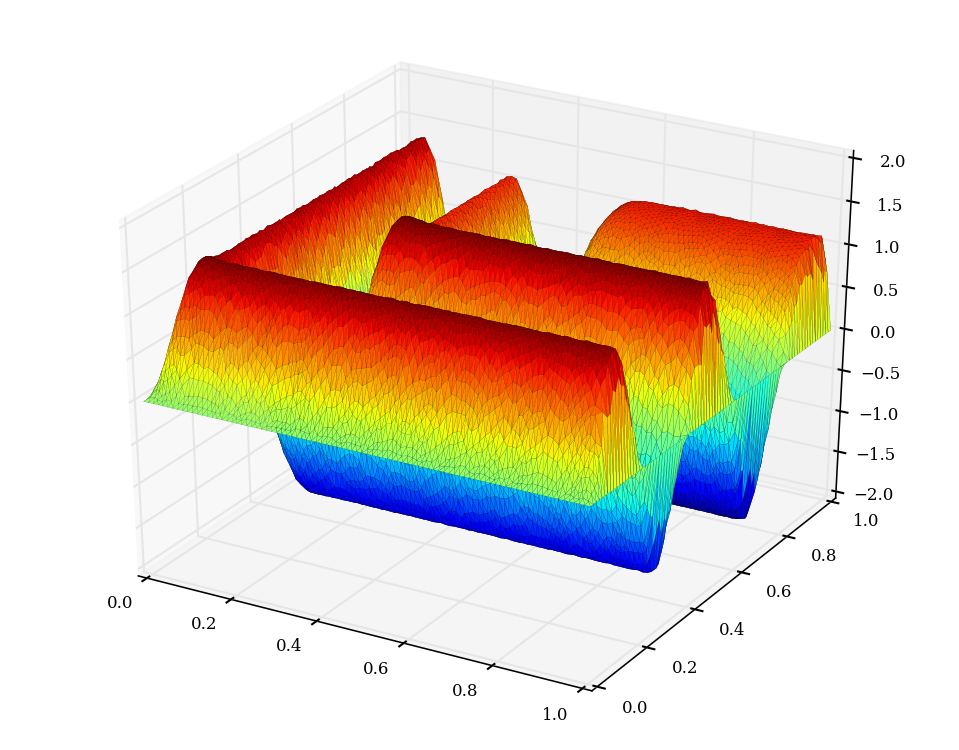
\includegraphics[width=3in]{Pictures/CDR/cdr_vector_5.png}

            Fifth POD vector.
        \end{center}
    \end{frame}

\section{A Little on SUPG}
    \begin{frame}
        \frametitle{Stabilization by Streamline Upwinding}
        \begin{equation}
            \varepsilon u_{xx} +
            u_x = 0,
            u(0) = 0, u(1) = 1
        \end{equation}
        \pause
        \begin{equation}
            \varepsilon \dfrac{U_{i + 1} - 2 U_i + U_{i - 1}}{h^2} +
            \dfrac{U_{i + 1} - U_{i - 1}}{2 h} = 1
        \end{equation}
        known to be an unstable discretization for small \(\varepsilon\)
        \pause
        \begin{align}
            \varepsilon
            \dfrac{U_{i + 1} - 2 U_i + U_{i - 1}}{h^2} +
            \dfrac{{\color{red} U_{i + 1}} - {\color{red} U_i}}{h} &= 1       \\
            \varepsilon
            \dfrac{U_{i + 1} - 2 U_i + U_{i - 1}}{h^2} +
            \dfrac{{\color{red} U_{i + 1}}}{2 h} +
            \dfrac{{\color{red} U_{i + 1}}}{2 h} -
            \dfrac{{\color{red} 2 U_i}}{2 h} +
            \dfrac{\color{red} U_{i - 1}}{2 h} +
            \dfrac{1}{2 h}
            \left(
            {{\color{red} U_{i - 1}} - {\color{red} U_{i - 1}}}
            \right)
            &= 1                                                              \\
            \left(\varepsilon + {\color{red} \dfrac{h}{2}}\right)
            \dfrac{U_{i + 1} - 2 U_i + U_{i - 1}}{h^2} +
            \dfrac{{\color{red} U_{i + 1}} - {\color{red} U_{i - 1}}}{2 h} &= 1
        \end{align}
        \pause
        Using a forward difference (\emph{upwinding}) results in an order \(1\)
        method with a much larger diffusion coefficient
    \end{frame}

    \begin{frame}
        \frametitle{Stabilization by Streamline Upwinding (Petrov-Galerkin)}
        We can get a similar result for Finite Elements with the Petrov-Galerkin
        method by choosing test functions \(\varphi + \delta \varphi_x\):
        \begin{align}
            \varepsilon ((\varphi + \delta \varphi_x)_x, u_x)
            + (\varphi + \delta \varphi_x, u_x)
            &= (\varphi + \delta \varphi_x, f)                                \\
            (\varepsilon + \delta) (\varphi_x, u_x)
            + \varepsilon \delta (\varphi_{xx}, u_x)
            + (\varphi, u_x)
            &= (\varphi + \delta \varphi_x, f)
        \end{align}
        so the new viscous length scale is \(O(\sqrt{\delta})\): if \(\delta =
        O(h)\) then this can be resolved.
    \end{frame}

    \begin{frame}
        \frametitle{Stabilization by SUPG}
        \begin{center}
            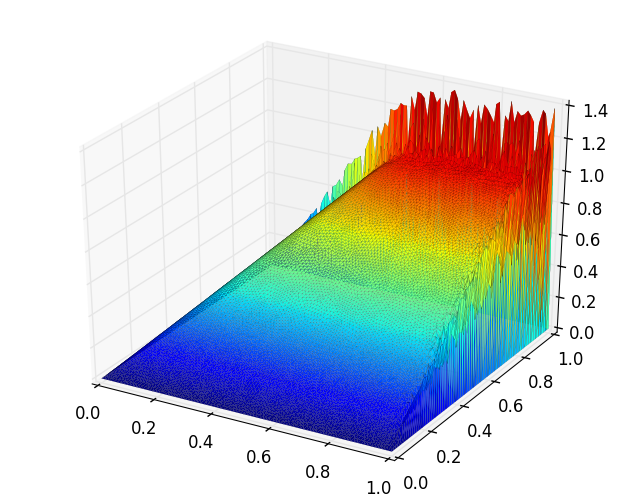
\includegraphics[width=3in]{Pictures/CDR/cdr_unstabilized.png}

            \(f = 1\), \(\varepsilon = 10^{-3}\), \(\vec{b} = (\cos(\pi/3),
            \sin(\pi/3))\), and \(c = 10^{-3}\): no stabilization.
        \end{center}
    \end{frame}

    \begin{frame}
        \frametitle{Stabilization by SUPG}
        \begin{center}
            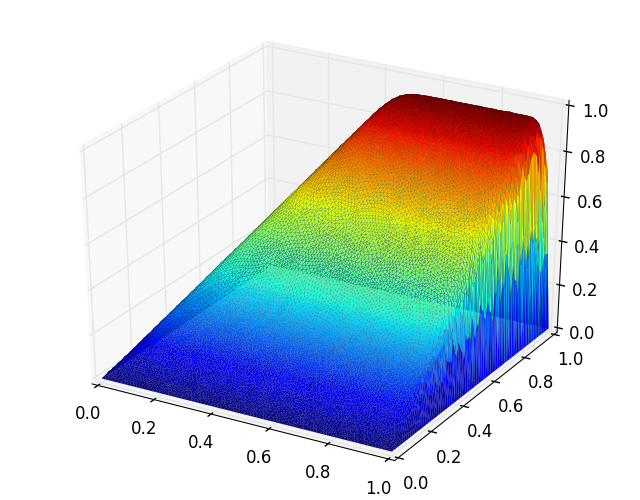
\includegraphics[width=3in]{Pictures/CDR/cdr_stabilized.png}

            \(f = 1\), \(\varepsilon = 10^{-3}\), \(\vec{b} = (\cos(\pi/3),
            \sin(\pi/3))\), and \(c = 10^{-3}\), with SUPG, \(\delta = h\).
        \end{center}
    \end{frame}

    \begin{frame}
        \frametitle{The SUPG-ROM}
        \begin{itemize}
            \item SUPG helps us avoid instabilities arising from unresolved
                  modes
                  \pause
            \item Unresolved modes \(\rightarrow\) aliasing onto the resolved
                  parts (wiggles)
                  \pause
            \item ROMs, by definition, have lots of unresolved modes!
        \end{itemize}
        \pause
        \emph{Plan:} add SUPG to a POD-ROM for the convection-diffusion-reaction
        equation, with analysis done with both FEM and POD estimates.
    \end{frame}

    \begin{frame}
    \frametitle{Error estimates}
    We assume a centered trajectory \(u_s\), ROM approximating the
    fluctuations \(u_r\), and projection onto the POD space \(P_r\):
    \begin{equation}
        \begin{aligned}
            u - (u_s + u_r) &= (u - P_r(u_h)) + (P_r(u_h) - (u_s + u_r))      \\
            &:= \eta - \phi_r
        \end{aligned}
    \end{equation}
    \pause
    Error estimate of the form (Giere, 2015 \cite{giere2015supg})
    \begin{equation}
        \begin{aligned}
            |||\phi_r|||_{\mathrm{SUPG}, r}
            \leq C
            \bigg[
            &\left(1 + \dfrac{1}{\sqrt{\delta}} + \sqrt{\delta}\right)
            \|\eta\|
            + \sqrt{\varepsilon} \|\nabla \eta\|                              \\
            &+ \sqrt{\delta} \|\vec{b} \cdot \nabla \eta\|
            + \sqrt{\delta} \sqrt{\sum_T \|\Delta \eta\|_{0,T}^2}
            \bigg].
        \end{aligned}
    \end{equation}
\end{frame}

\begin{frame}
    \frametitle{The POD Option}
    Seminorm bound on derivatives: \cite{iliescu2013variational, singler2014new}
    \begin{equation}
        \snapsum \Seminorms{u_n - \sum_{j = 0}^{r - 1} \inl{j} \phi_j}_s^2
        = \remainder{j} \Seminorms{\phi_j}_s^2 \sigma_j^2.
    \end{equation}

    %% TODO what was C_1 again? Its not in my old slides.
    \begin{align}
        \Norm{\eta} &\leq C_1 \sqrt{\remainder{j} \sigma_j^2}
        := C_1 \Lambda_0                                                      \\
        \Norm{\nabla \eta}
        &\leq C_1 \sqrt{\remainder{j} \sigma_j^2 \Seminorm{\varphi_j}_1}
        := C_1 \Lambda_1                                                      \\
        \sqrt{\sumT \Norm{\delta \eta}_T^2}
        &\leq C_1 \sqrt{\remainder{j} \sigma_j^2 \Seminorm{\varphi_j}_2}
        := C_1 \Lambda_2.
    \end{align}

    \pause
    \begin{equation}
        \delta = \dfrac{\Lambda_{0}}{\Lambda_{2} \varepsilon + \Lambda_{0} +
        \Lambda_{1}}.
    \end{equation}
\end{frame}

\begin{frame}
    \frametitle{The Finite Element Option}
    Another option is to use finite element estimates \cite{roos2008robust} with
    order \(m\) polynomials and \(s\) derivatives:
    \begin{equation}
        | \eta |_s \leq C h^{m + 1/2 - s}
    \end{equation}

    Solve the optimization problem for \(\delta\):
    \begin{equation}
        \delta = \frac{\Lambda_{0} h^{2} + h^{m + \frac{5}{2}}}{{\left(h^{2}
        + \varepsilon + h\right)} \Lambda_{0} + \varepsilon h^{m + \frac{1}{2}} +
        h^{m + \frac{5}{2}} + h^{m + \frac{3}{2}}}
    \end{equation}
    \pause
    If \(m \geq 2\):
    \begin{equation}
        \delta \approx \dfrac{\Lambda_0 h^2}{h \Lambda_0} = h
    \end{equation}
    We are back where we started! In practice the two stabilization parameters
    are within about \(10\%\).
\end{frame}

\section{Numerical Results}
    \begin{frame}
        \frametitle{POD-ROM and SUPG-ROM}
        \begin{center}
            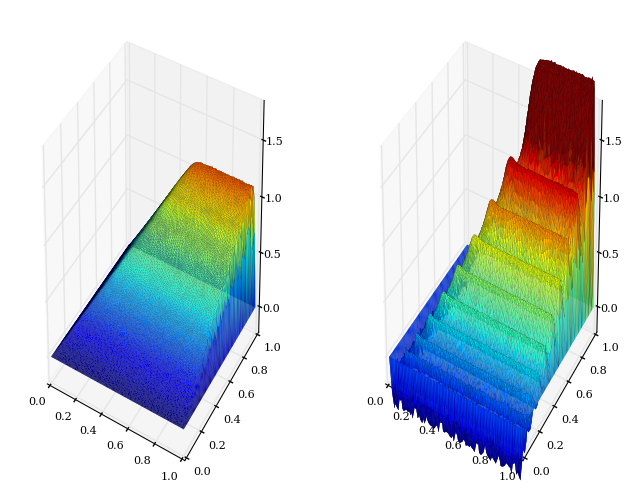
\includegraphics[width=3in]{Pictures/CDR/codina_rising_wave_10.png}

            Stabilized (left) and unstabilized (right) POD-ROMs at \(t = 1.0\).
        \end{center}
    \end{frame}

    \begin{frame}
        \frametitle{Comparison of POD coefficients}
        \begin{center}
            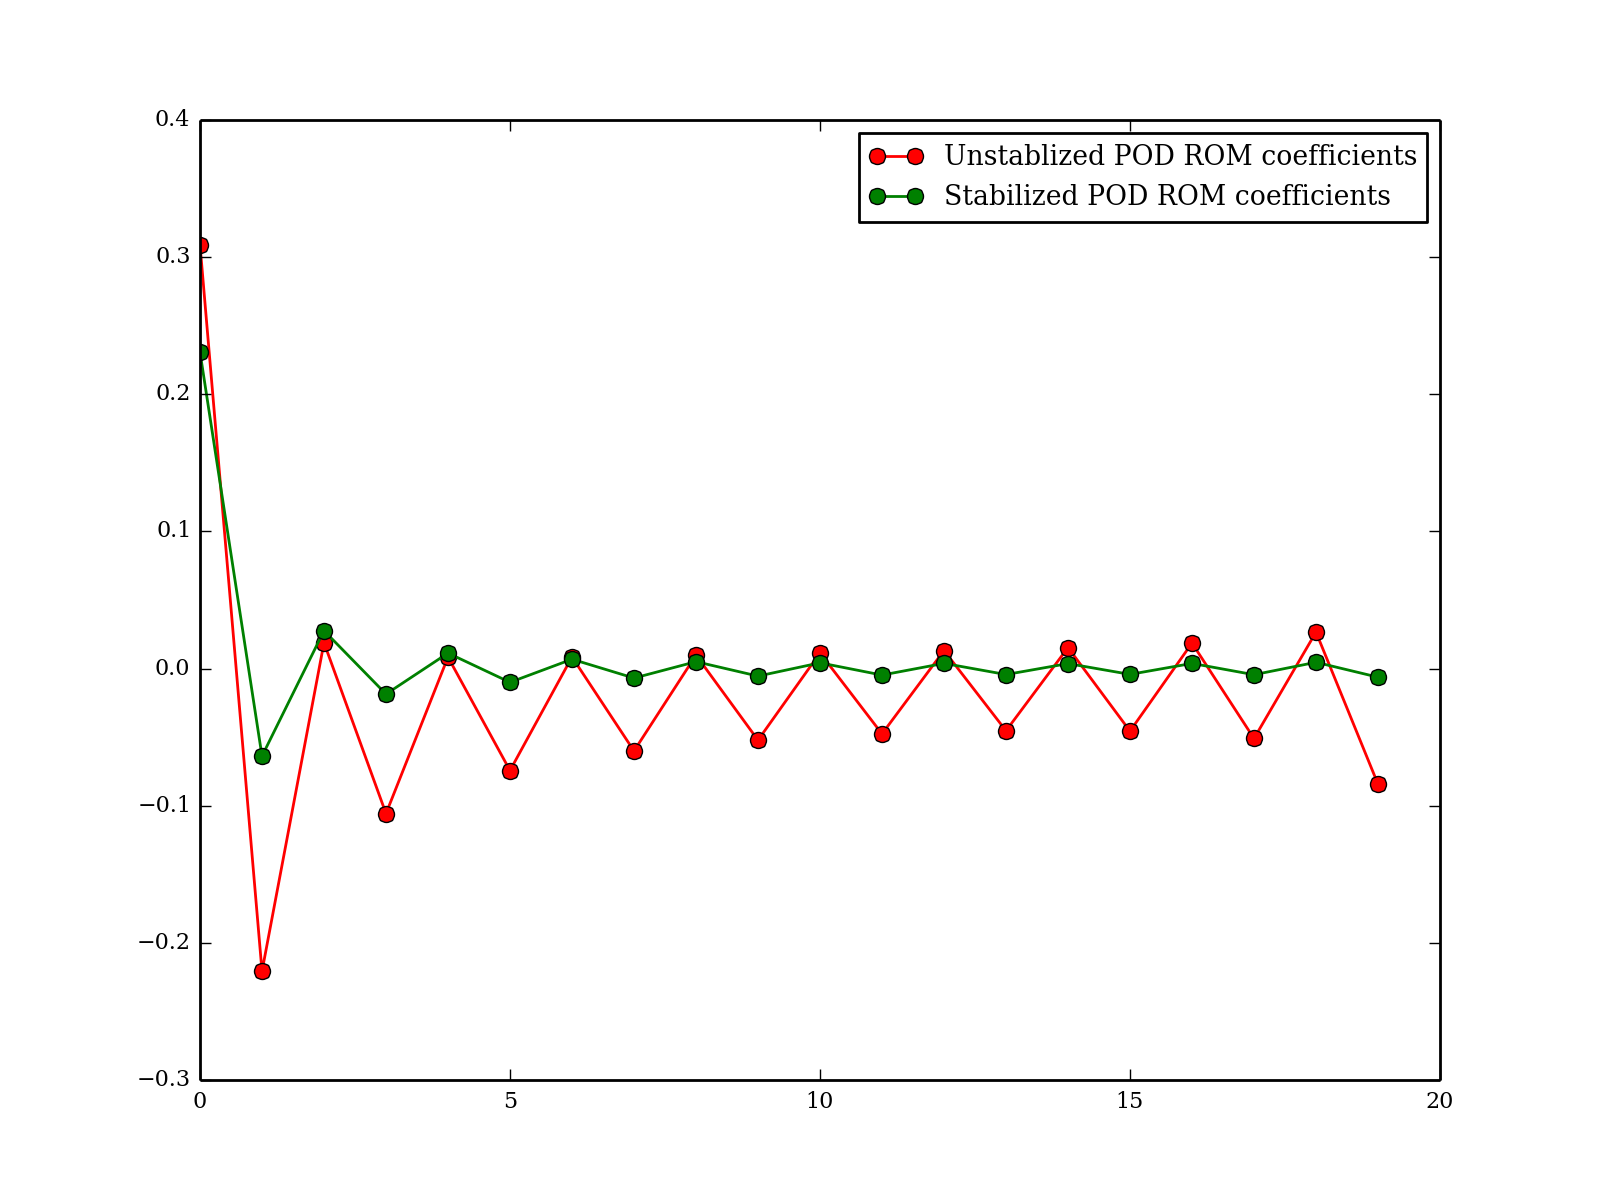
\includegraphics[width=3in]{Pictures/CDR/codina_rising_wave_coefficients_10.png}

            Coefficients at \(t = 1.0\) for the stabilized and unstabilized models.
        \end{center}
    \end{frame}

\section{Summary}
    \begin{frame}
        \frametitle{Summary}
        \begin{itemize}
            \item ROMs for convection-dominated problems have aliasing issues
                  when scales are unresolved.
            \item We can overcome this problem with SUPG; tentatively, this
                  implies that the usual FEM stabilization methods may be
                  useful.
        \end{itemize}
    \end{frame}

    \begin{frame}
        \begin{center}
            \textcolor{RPIred}{\Huge Thank You!}
        \end{center}
    \end{frame}


\begin{frame}[allowframebreaks]
    \bibliographystyle{plain}
    \tiny
    {
    \bibliography{citations}
    }
\end{frame}
\end{document}
